% !TeX root = markov.tex

%%%%%%%%%%%%%%%%%%%%%%%%%%%%%%%%%%%%%%%%%%%%%%%%%%%%%%%%%%%%%%%%

\documentclass[11pt,a4paper]{article}

\usepackage{mathpazo}
\usepackage{microtype}
\usepackage{url}
\usepackage{graphicx}

% TikZ package
\usepackage{tikz}
\usetikzlibrary{arrows.meta}
\usetikzlibrary{positioning}
\usetikzlibrary{automata}
\tikzset {>=Stealth}

% Displaystyle for fractions and combinations
\newcommand*{\disfrac}[2]{\displaystyle\frac{#1}{#2}}
\newcommand*{\dischoose}[2]{\displaystyle{#1 \choose #2}}
\newcommand*{\sm}[1]{$\scriptstyle #1$}
\setcounter{tocdepth}{1}

% Change LaTeX defaults for figures
\renewcommand{\topfraction}{0.9}
\renewcommand{\bottomfraction}{0.8}
\setcounter{topnumber}{1}
\setcounter{bottomnumber}{2}
\setcounter{totalnumber}{3}
\renewcommand{\textfraction}{0.07}
\renewcommand{\floatpagefraction}{0.7}

% Layout
\textwidth=150mm
\textheight=225mm
\topmargin=0pt
\headheight=11pt
\oddsidemargin=1em
\evensidemargin=0mm
\headsep=0pt
\parindent=0pt
\renewcommand{\baselinestretch}{1.1}
\setlength{\parskip}{0.3\baselineskip plus 1pt minus 1pt}

%\includeonly{markov-maze}

\begin{document}

%% !TeX root = markov.tex

\thispagestyle{empty}

\begin{center}
\textbf{\LARGE Markov Chain Simulations}

\bigskip
\bigskip
\bigskip

\textbf{\Large Moti Ben-Ari}

\bigskip

\url{http://www.weizmann.ac.il/sci-tea/benari/}

\bigskip
\bigskip
\bigskip

\today

\end{center}

\vfill

\begin{center}
\copyright{} Moti Ben-Ari $2023$
 \end{center}
 
\begin{small}
This work is licensed under Attribution-ShareAlike 4.0 International. To view a copy of this license, visit \url{http://creativecommons.org/licenses/by-sa/4.0/}.
\end{small}
\newpage

\tableofcontents

\newpage

\section{Introduction}

Simulations are an excellent way of understanding probability, especially, the behavior of processes of long duration. Simulation programs enable the user to perform experiments by varying the parameters of problems interactively and analyzing the results, both printed and displayed in graphs. The simulations in this archive are of processes known as \emph{Markov chains}, where the next state of the system depends only on the current state and not on the history of how the process got to the current state. 

The following problems are simulated: the \emph{gambler's ruin} in 
Section~\ref{s.gamblers}, one-, two- and three-dimensional \emph{random walk} in Section~\ref{s.walk}, the \emph{Ehrenfest model} in Section~\ref{s.ehrenfest} and the \emph{two-state process} in Section~\ref{s.two-state}.

\subsection*{Technical notes}

The programs are written in the Python 3 language and use the \verb+matplotlib+ library to generate the graphs. You need to install Python (\url{https://www.python.org/downloads/}) although a knowledge of Python programming is not necessary to run the simulations.

To run in the IDLE or Thonny environments, change the configuration constant \verb+CLOSE+ to \verb+True+. When the simulation is run multiple times, you will have to close each figure before running a new simulation. This is not necessary if the programs are run in the Visual Studio Code environment or from the command line.

Parameters directly related to the problems, such as the probability of success, can be modified interactively. Others, related to the simulation, such as the number of steps in a simulation, are defined in a module \verb+configuration.py+ which just contains declarations of values so it is easy to modify. The code that uses \verb+matplotlib+ appears in a separate module.

\subsection*{Sources}

A knowledge of probability is assumed at the level of the first few chapters of \cite{BW,ross}. These textbooks include examples of the gambler's ruin and random walk, as well as short presentations of Markov chains. The clearest explanational of one-dimensional random walk is in \cite{border}. I was introduced to these problems by Mosteller \cite{mosteller}; my ``reworking'' of this book is in \cite{mos}. A comprehensive work on Markov chains is \cite{privault} from which I took most of the theoretical results.

%% !TeX root = markov.tex

\section{Gambler's ruin}\label{s.gamblers}

\textbf{Problem} Two players $A$ and $B$ compete in a contest. There is an initial finite capital of $n$ units: $A$ has $i$ and $B$ has $n-i$. They repeatedly play a game where the probability that $A$ wins is $p$ and the probability that $B$ wins is $q=1-p$. The loser gives one unit to the winner. When one player has all $n$ units the contest is terminated and that player is declared the winner.
\begin{enumerate}
\item Given initial parameters $(p, n, i)$, what is the probability that $A$ wins?
\item What is the expected duration of the game?
\end{enumerate}
\begin{center}
\begin{tikzpicture}[scale=1.2]
\draw (0,0) node[above left] {$A$} -- 
      (10,0) node[above right] {$B$};
\foreach \x in {0,1,2,3,4,5,6,7,8,9,10} {
  \draw (\x,0) -- +(0,4pt);
  \node at (\x,-10pt) { $\x$ };
}
\node at (4,-9mm) {$i$};
\node at (10,-9mm) {$n$};
\draw[fill] (4,7mm) circle[radius=1pt];
\draw[->] (4,7mm) -- node[above] {$q$} +(-1,0);
\draw[->] (4,7mm) -- node[above] {$p$} +(1,0);
\end{tikzpicture}
\end{center}

\subsection{Theoretical results}

Given $(p,n,i)$ the probability that $A$ wins the contest is:
\[
P_A(p, n, i) = \left(\frac{1-r^{i}}{1-r^n}\right)\,,
\]
where $r=q/p$. By symmetry, the probability that $B$ wins is:
\[
P_B(p, n, i) = \left(\frac{1-(1/r)^{n-i}}{1-(1/r)^{n}}\right)\,.
\]

For $p\neq 1/2$ the expected duration of the contest is:
\[
E_{\mathit{duration}}(p,n,i)=\frac{1}{q-p}\left(i-n
\frac{1-r^k}{1-r^n}\right)\,,
\]
while for $p=1/2$ the expected duration of the contest is:
\[
E_{\mathit{duration}}(p,n,i)=i(n-1)\,.
\]
Of course the duration does not depend on which player wins. If $A$ wins, the contest terminates for $B$ also, and conversely.

\subsection{Running the simulations}

The program asks the user how to run the simulations and then runs them in a loop. You can run the same simulation again with the saved parameters, enter new parameters, or run a sequence of simulations for a range of probabilities or initial values. Here is an output for $10000$ simulations:
\begin{verbatim}
Probability = 0.45, capital = 20, initial = 8
Wins = 789, losses = 9211, limits exceeded = 0
Proportion of wins     = 0.0789
Probability of winning = 0.0732
Average duration  = 65
Expected duration = 65
\end{verbatim}
A graph of the proportion of wins and the histogram of the durations are shown in Figures~\ref{f.gambler-hist1}, \ref{f.gambler-hist2}. The vertical lines are the average durations.

\begin{figure}
\begin{center}
\includegraphics[width=\textwidth]{gamblers-ruin-01}
\caption{Proportion of wins and histogram for $n=20, i=10$ and multiple probabilities}\label{f.gambler-hist1}
\end{center}
\end{figure}

\begin{figure}
\begin{center}
\includegraphics[width=\textwidth]{gamblers-ruin-02}
\caption{Proportion of wins and histogram for $p=0.45, n=20$ and multiple initial values}\label{f.gambler-hist2}
\end{center}
\end{figure}

%\include{markov-walk}
%% !TeX root = markov.tex

\section{The Ehrenfest model}\label{s.ehrenfest}

\textbf{Problem} The Ehrenfest model is designed to model diffusion of particles between two containers. In the following diagram there are four particles in the left container and six particles in the right container for a total of $n=10$ particles:
\begin{center}
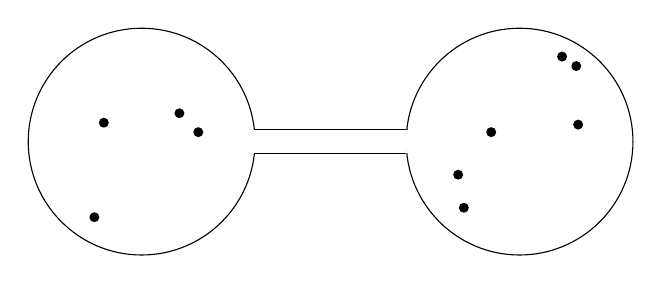
\begin{tikzpicture}[scale=1.2]
\draw (0,0) node {} circle[radius=1.2];
\draw[white,thick] (-6:1.2) arc(-6:6:1.2);
\draw (-6:1.2) -- +(1.63,0);
\draw (6:1.2) -- +(1.63,0);
\fill (-.4,.2) circle[radius=1.5pt];
\fill (.4,.3) circle[radius=1.5pt];
\fill (-.5,-.8) circle[radius=1.5pt];
\fill (.6,.1) circle[radius=1.5pt];
\begin{scope}[xshift=4cm]
\draw (0,0) node {} circle[radius=1.2];
\draw[white,thick] (174:1.2) arc(174:186:1.2);
\fill (-.3,.1) circle[radius=1.5pt];
\fill (.45,.9) circle[radius=1.5pt];
\fill (-.65,-.35) circle[radius=1.5pt];
\fill (.62,.18) circle[radius=1.5pt];
\fill (-.59,-.7) circle[radius=1.5pt];
\fill (.6,.8) circle[radius=1.5pt];
\end{scope}
\end{tikzpicture}
\end{center}
Repeated choose a particle at random with uniform distribution and move it to the other container. If there are $i$ particles in the left container then the probability of choosing a particle from the left container is $i/n$ and the probability of choosing a particle from the right container is $(n-i)/n$. If one container is empty the next particle must be chosen from the other container. 

The problem is similar to the gambler's ruin except that: (a) the process never ends and (b) the probability of a left or right step changes with each step:
\begin{center}
\begin{tikzpicture}[scale=1.2]
\draw (0,0) node[above left] {$A$} -- 
      (10,0) node[above right] {$B$};
\foreach \x in {0,1,2,3,4,5,6,7,8,9,10} {
  \draw (\x,0) -- +(0,4pt);
  \node at (\x,-10pt) { $\x$ };
}
\node at (4,-9mm) {$i$};
\node at (10,-9mm) {$n$};
\draw[fill] (4,7mm) circle[radius=1pt];
\draw[->] (4,7mm) -- node[above,xshift=-8pt] {$(n-i)/n$} +(-1,0);
\draw[->] (4,7mm) -- node[above,xshift=2pt] {$i/n$} +(1,0);
\draw[->] (0,7mm) -- node[above] {$1$} +(1,0);
\draw[<-] (9,7mm) -- node[above] {$1$} +(1,0);
\end{tikzpicture}
\end{center}

\subsection{Theoretical results}

The process is a Markov chain which eventually reaches a \emph{stationary distribution}:
\[
s_i=\dischoose{n}{i}\left(\frac{1}{n}\right)^n\,,
\]
where $s_i$ is the proportion of time that the particle is at the $i$'th position.

\subsection{Running the simulations}

The program asks the user how to run the simulation: with the saved value of $n$ or with a new value of $n$. Here is an output of the simulation:
\begin{verbatim}
Total particles in urns = 10
Theoretical stationary distribution
[0.001 0.01  0.044 0.117 0.205 0.246 0.205 0.117 0.044 0.01  0.001]
Simulation stationary distribution
[0.001 0.009 0.044 0.12  0.208 0.243 0.205 0.121 0.042 0.008 0.001]
\end{verbatim}
A graph of these distributions is shown in Figure~\ref{f.ehrenfest1}; the theoretical distribution and the result of simulation are so close together that the lines are slightly offset.

\begin{figure}
\begin{center}
\includegraphics[width=\textwidth]{ehrenfest-01}
\caption{Stationary distribution for the Ehrenfest model}\label{f.ehrenfest1}
\end{center}
\end{figure}


%% !TeX root = markov.tex

\section{The two-state process}\label{s.two-state}

The two-state process is similar to the Ehrenfest model in that the probabilities at each step are different and we are interested in the stationary probability distribution of the unbounded process. There are two states $A,B$. In state $A$ the process transitions to $B$  with probability $a$ and remains in $A$ with probability $1-a$. Similarly, the probability of a transition from $B$ to $A$ is $b$ and the probability of remaining in $B$ is $1-b$.
\begin{center}
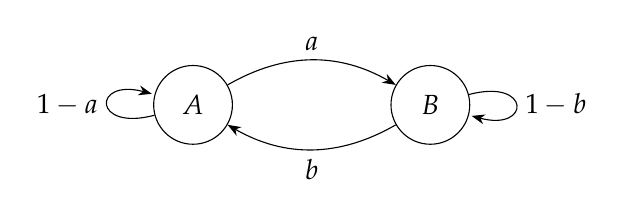
\begin{tikzpicture}[->,node distance = 6mm and 2cm]
\node[draw,circle,minimum size=10mm] (A) {$A$};
\node[draw,circle,minimum size=10mm] (B) [right=of A] {$B$};
\draw (A) edge[bend left] node[above] {$a$} (B);
\draw (B) edge[bend left] node[below] {$b$} (A);
\draw (A) edge [loop left] node {$1-a$} (A);
\draw (B) edge [loop right] node {$1-b$} (B);
\end{tikzpicture}
\end{center}
The stationary distribution, that is, the proportion of visits to $A$ and to $B$ is:
\[
\left[\frac{b}{a+b}, \frac{a}{a+b}\right]\,.
\]
Here is an output of a simulation:
\begin{verbatim}
Probabilities:  a = 0.500, b = 0.333
Theoretical stationary distribution: A = 0.400, B = 0.600
Simulation  stationary distribution: A = 0.402, B = 0.598
\end{verbatim}
When $a+b=1$ the probability of being at $A$ is $b$ and the probability of being at $B$ is $a$:
\begin{verbatim}
Probabilities:  a = 0.333, b = 0.667
Theoretical stationary distribution: A = 0.667, B = 0.333
Simulation  stationary distribution: A = 0.674, B = 0.326
\end{verbatim}
You can enter a required proportion $p$ of visits to $B$ and any probability $0<a<p$. The proportion will be achieved for:
\[
b = \frac{a(1-p)}{p}\,,
\]
as shown in the following simulation where we entered $p=0.8, a=0.6$:
\begin{verbatim}
Probabilities:  a = 0.600, b = 0.150, proportion = 0.800
Theoretical stationary distribution: A = 0.200, B = 0.800
Simulation  stationary distribution: A = 0.194, B = 0.806
\end{verbatim}

%\include{markov-maze}
%% !TeX root = markov.tex

\addcontentsline{toc}{section}{References}

\bibliographystyle{plain}
\bibliography{markov}


%%%%%%%%%%%%%%%%%%%%%%%%%%%%%%%%%%%%%%%%%%%%%%%%%%%%%%%%%%%%%%%%%%%%%

\thispagestyle{empty}

\begin{center}
\textbf{\LARGE Markov Chain Simulations}

\bigskip
\bigskip
\bigskip

\textbf{\Large Moti Ben-Ari}

\bigskip

\url{http://www.weizmann.ac.il/sci-tea/benari/}

\bigskip
\bigskip
\bigskip

\today

\end{center}

\vfill

\begin{center}
\copyright{} Moti Ben-Ari $2023$
 \end{center}
 
\begin{small}
This work is licensed under Attribution-ShareAlike 4.0 International. To view a copy of this license, visit \url{http://creativecommons.org/licenses/by-sa/4.0/}.
\end{small}
\newpage

\tableofcontents

\newpage

%%%%%%%%%%%%%%%%%%%%%%%%%%%%%%%%%%%%%%%%%%%%%%%%%%%%%%%%%%%%%%%%%%%%%


\section{Introduction}

Simulations are an excellent way of understanding probability, especially, the behavior of processes of long duration. Simulation programs enable the user to perform experiments by varying the parameters of problems interactively and analyzing the results, both printed and displayed in graphs. The simulations in this archive are of processes known as \emph{Markov chains}, where the next state of the system depends only on the current state and not on the history of how the process got to the current state. 

The following problems are simulated: the \emph{gambler's ruin} in 
Section~\ref{s.gamblers}, one-, two- and three-dimensional \emph{random walk} in Section~\ref{s.walk}, the \emph{Ehrenfest model} in Section~\ref{s.ehrenfest} and the \emph{two-state process} in Section~\ref{s.two-state}.

\subsection*{Technical notes}

The programs are written in the Python 3 language and use the \verb+matplotlib+ library to generate the graphs. You need to install Python (\url{https://www.python.org/downloads/}) although a knowledge of Python programming is not necessary to run the simulations.

To run in the IDLE or Thonny environments, change the configuration constant \verb+CLOSE+ to \verb+True+. When the simulation is run multiple times, you will have to close each figure before running a new simulation. This is not necessary if the programs are run in the Visual Studio Code environment or from the command line.

Parameters directly related to the problems, such as the probability of success, can be modified interactively. Others, related to the simulation, such as the number of steps in a simulation, are defined in a module \verb+configuration.py+ which just contains declarations of values so it is easy to modify. The code that uses \verb+matplotlib+ appears in a separate module.

\subsection*{Sources}

A knowledge of probability is assumed at the level of the first few chapters of \cite{BW,ross}. These textbooks include examples of the gambler's ruin and random walk, as well as short presentations of Markov chains. The clearest explanational of one-dimensional random walk is in \cite{border}. I was introduced to these problems by Mosteller \cite{mosteller}; my ``reworking'' of this book is in \cite{mos}. A comprehensive work on Markov chains is \cite{privault} from which I took most of the theoretical results.

%%%%%%%%%%%%%%%%%%%%%%%%%%%%%%%%%%%%%%%%%%%%%%%%%%%%%%%%%%%%%%%%%%%%%

\section{Gambler's ruin}\label{s.gamblers}

\textbf{Problem} Two players $A$ and $B$ compete in a contest. There is an initial finite capital of $n$ units: $A$ has $i$ and $B$ has $n-i$. They repeatedly play a game where the probability that $A$ wins is $p$ and the probability that $B$ wins is $q=1-p$. The loser gives one unit to the winner. When one player has all $n$ units the contest is terminated and that player is declared the winner.
\begin{enumerate}
\item Given initial parameters $(p, n, i)$, what is the probability that $A$ wins?
\item What is the expected duration of the game?
\end{enumerate}
\begin{center}
\begin{tikzpicture}[scale=1.2]
\draw (0,0) node[above left] {$A$} -- 
      (10,0) node[above right] {$B$};
\foreach \x in {0,1,2,3,4,5,6,7,8,9,10} {
  \draw (\x,0) -- +(0,4pt);
  \node at (\x,-10pt) { $\x$ };
}
\node at (4,-9mm) {$i$};
\node at (10,-9mm) {$n$};
\draw[fill] (4,7mm) circle[radius=1pt];
\draw[->] (4,7mm) -- node[above] {$q$} +(-1,0);
\draw[->] (4,7mm) -- node[above] {$p$} +(1,0);
\end{tikzpicture}
\end{center}

\subsection{Theoretical results}

Given $(p,n,i)$ the probability that $A$ wins the contest is:
\[
P_A(p, n, i) = \left(\frac{1-r^{i}}{1-r^n}\right)\,,
\]
where $r=q/p$. By symmetry, the probability that $B$ wins is:
\[
P_B(p, n, i) = \left(\frac{1-(1/r)^{n-i}}{1-(1/r)^{n}}\right)\,.
\]

For $p\neq 1/2$ the expected duration of the contest is:
\[
E_{\mathit{duration}}(p,n,i)=\frac{1}{q-p}\left(i-n
\frac{1-r^k}{1-r^n}\right)\,,
\]
while for $p=1/2$ the expected duration of the contest is:
\[
E_{\mathit{duration}}(p,n,i)=i(n-1)\,.
\]
Of course the duration does not depend on which player wins. If $A$ wins, the contest terminates for $B$ also, and conversely.

\subsection{Running the simulations}

The program asks the user how to run the simulations and then runs them in a loop. You can run the same simulation again with the saved parameters, enter new parameters, or run a sequence of simulations for a range of probabilities or initial values. Here is an output for $10000$ simulations:
\begin{verbatim}
Probability = 0.45, capital = 20, initial = 8
Wins = 789, losses = 9211, limits exceeded = 0
Proportion of wins     = 0.0789
Probability of winning = 0.0732
Average duration  = 65
Expected duration = 65
\end{verbatim}
A graph of the proportion of wins and the histogram of the durations are shown in Figures~\ref{f.gambler-hist1}, \ref{f.gambler-hist2}. The vertical lines are the average durations.

\begin{figure}
\begin{center}
\includegraphics[width=\textwidth]{gamblers-ruin-01}
\caption{Proportion of wins and histogram for $n=20, i=10$ and multiple probabilities}\label{f.gambler-hist1}
\end{center}
\end{figure}

\begin{figure}
\begin{center}
\includegraphics[width=\textwidth]{gamblers-ruin-02}
\caption{Proportion of wins and histogram for $p=0.45, n=20$ and multiple initial values}\label{f.gambler-hist2}
\end{center}
\end{figure}

%%%%%%%%%%%%%%%%%%%%%%%%%%%%%%%%%%%%%%%%%%%%%%%%%%%%%%%%%%%%%%%%%%%%%

\section{Random walk}\label{s.walk}

\textbf{Problem} A particle is placed at the origin of the $x$-axis. It repeatedly takes steps: right with probability $p$ and left with probability $q=1-p$.
\begin{enumerate}
\item What is the probability that the particle will return to the origin?
\item What is the expected duration until the particle returns to the origin?
\end{enumerate}
\begin{center}
\begin{tikzpicture}[scale=1.2]
\draw[<->] (-6,0) -- (6,0);
\foreach \x in {-5,-4,-3,-2,-1,0,1,2,3,4,5} {
  \draw (\x,0) -- +(0,4pt);
  \node at (\x,-10pt) { $\x$ };
}
\node at (-6,-10pt) { $\cdots$ };
\node at (6,-10pt) { $\cdots$ };
\draw[fill] (0,7mm) circle[radius=1pt];
\draw[->] (0,7mm) -- node[above] {$q$} +(-1,0);
\draw[->] (0,7mm) -- node[above] {$p$} +(1,0);
\end{tikzpicture}
\end{center}

\subsection{Theoretical results}

By symmetry let the first step be to the right. The particle can only return to the origin after an even number of steps. Assume that $p=1/2$. Let $S_{2m}$ be the position of the particle after $2m$ steps. Then:
\[
P(S_{2m}=0) = \dischoose{2m}{m}\disfrac{1}{2^{2m}}\,,
\]
which by Stirling's formula is:
\[
P(S_{2m}=0) \approx \disfrac{1}{\sqrt{\pi m}}\,.
\]
It can now be proved that the probability of a return to the origin is $1$.

For $p\leq 1/2$, $P_{\mathit{origin}}$, the probability of a return to the origin, is $1$ and for $p\geq 1/2$ the probability is (Figure~\ref{f.walk1}):
\[
P_{\mathit{origin}} = \disfrac{q}{p}=\disfrac{1-p}{p}\,.
\]
\begin{figure}
\begin{center}
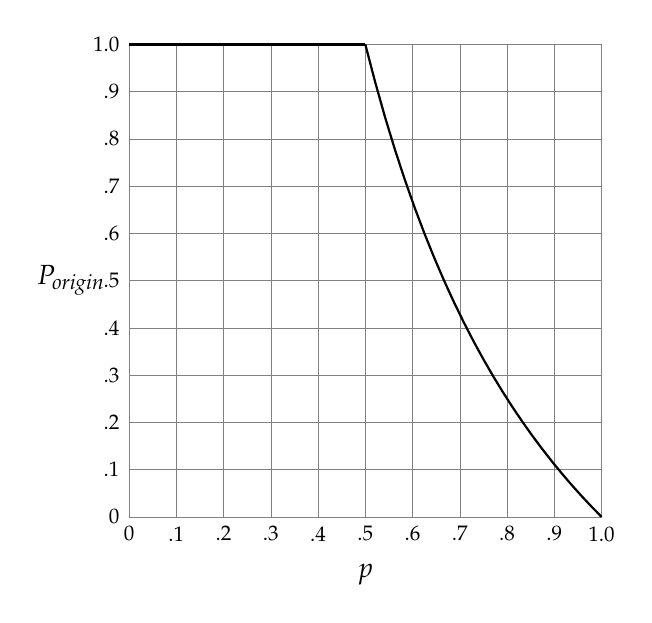
\begin{tikzpicture}[scale=6]
\draw[help lines,step=.1] (0,0) grid (1,1);
\foreach \x in {0,.1,.2,.3,.4,.5,.6,.7,.8,.9,1.0}
  \node[below] at (\x,0) {$\scriptstyle \x$};
\foreach \y in {0,.1,.2,.3,.4,.5,.6,.7,.8,.9,1.0}
  \node[left] at (0,\y) {$\scriptstyle \y$};
\draw[domain=0:.5,thick] plot (\x,1);
\draw[domain=.5:1,thick] plot (\x,{(1-\x)/\x});
\node at (.5,-3.5pt) {$p$};
\node at (-3.5pt,.5) {$P_{\mathit{origin}}$};
\end{tikzpicture}
\caption{Graph of $P_{\mathit{origin}}$}\label{f.walk1}
\end{center}
\end{figure}

$E_{\mathit{origin}}$, the expected duration until the first return to the origin, is infinite for $p\geq 1/2$ while for $p<1/2$ it is:
\[
E_{\mathit{origin}}=\disfrac{1}{q-p}=\disfrac{1}{1-2p}\,.
\]

\subsection{Running the simulations}

The program asks the user how to run the simulations and then runs them in a loop. You can run the same simulation again with the saved parameters, enter new parameters, or run a sequence of simulations for a range of probabilities or limits. Here is an output of the simulation:
\begin{verbatim}
Probability = 0.50, step limit   = 1000
Proportion returning to origin   = 0.977
Probability of return to origin  = 1.000
Proportion reaching limit        = 0.023
Mean duration (steps)            = 49
Expected duration (steps)        = infinity
\end{verbatim}
The proportion of wins in the simulation are very close to the theoretical probability, but the mean duration is far from infinite because the step limit was too small.  The proportion of wins and the mean durations are shown in Figures~\ref{f.random-walk-01} and \ref{f.random-walk-02}.
\begin{figure}
\begin{center}
\includegraphics[width=\textwidth]{random-walk-01}
\caption{Proportion of returns to origin and and mean durations for multiple probabilities}\label{f.random-walk-01}
\end{center}
\end{figure}
\begin{figure}
\begin{center}
\includegraphics[width=\textwidth]{random-walk-02}
\caption{Proportion of returns to origin and mean durations for multiple limits}\label{f.random-walk-02}
\end{center}
\end{figure}

\subsection{Two-dimensional random walk}

In a two-dimensional random walk a step of the particle consists of one step left or right on the $x$-axis with probability $1/2$ and simultaneously one step up or down on the $y$-axis also with probability $1/2$ (Figure~\ref{f.2d-random-walk}).

\begin{figure}
\begin{center}
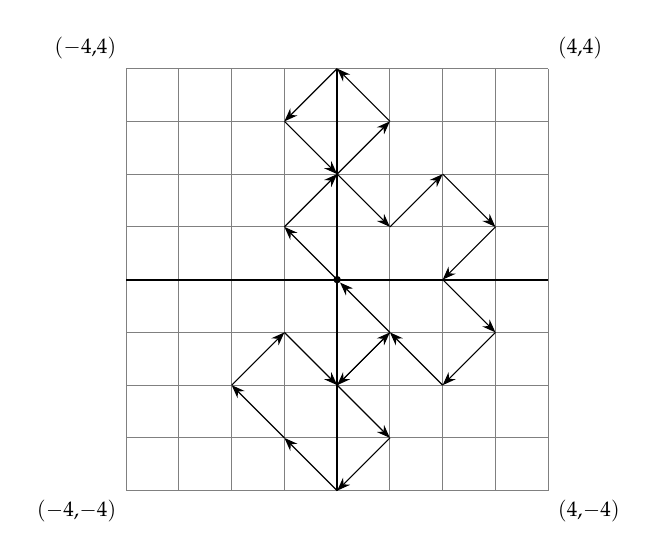
\begin{tikzpicture}[scale=.67]
\draw[color=gray] (-4,-4) grid (4,4);
\draw[thick] (-4,0) -- (4,0);
\draw[thick] (0,-4) -- (0,4);
\node[below left] at (-4,-4) {$\scriptstyle (-4,-4)$};
\node[below right] at (4,-4) {$\scriptstyle (4,-4)$};
\node[above left] at (-4,4) {$\scriptstyle (-4,4)$};
\node[above right] at (4,4) {$\scriptstyle (4,4)$};
\fill (0,0) circle[radius=2pt];
\draw[->] (0,0)  -- (-1,1);
\draw[->] (-1,1) -- (0,2);
\draw[->] (0,2)  -- (1,3);
\draw[->] (1,3)  -- (0,4);
\draw[->] (0,4)  -- (-1,3);
\draw[->] (-1,3) -- (0,2);
\draw[->] (0,2)  -- (1,1);
\draw[->] (1,1)  -- (2,2);
\draw[->] (2,2)  -- (3,1);
\draw[->] (3,1)  -- (2,0);
\draw[->] (2,0)  -- (3,-1);
\draw[->] (3,-1) -- (2,-2);
\draw[->] (2,-2) -- (1,-1);
\draw[->] (1,-1) -- (0,-2);
\draw[->] (0,-2) -- (1,-3);
\draw[->] (1,-3) -- (0,-4);
\draw[->] (0,-4) -- (-1,-3);
\draw[->] (-1,-3)-- (-2,-2);
\draw[->] (-2,-2)-- (-1,-1);
\draw[->] (-1,-1)-- (0,-2);
\draw[->] (0,-2) -- (1,-1);
\draw[->] (1,-1) -- (.055,-.055);
\end{tikzpicture}
\end{center}
\caption{A $22$-step two-dimensional random walk}\label{f.2d-random-walk}
\end{figure}
The probability $1$ the particle will return to the origin but the expected duration is infinite! Therefore, when you run the simulation with any reasonable limit on the number of steps, the proportion of returns to the origin will be much less than $1$ and the mean duration will be quite large:
\begin{verbatim}
Limit                            = 100000
Proportion returning to origin   = 0.777
Proportion reaching limit        = 0.223
Mean duration (steps)            = 24133
\end{verbatim}

The program structure is the same as for the one-dimensional random walk. You can enter the step limit parameter for each simulation interactively and can run the simulations for a range of limits expressed as percentages of the parameter. Figure~\ref{f.random-walk-2D} shows the proportion of returns to the origin and the mean durations for a range of limits.

\begin{figure}
\begin{center}
\includegraphics[width=\textwidth]{random-walk-02}
\caption{Proportion of returns to origin and and mean durations for multiple limits}\label{f.random-walk-2D}
\end{center}
\end{figure}

\subsection{Three-dimensional random walk}

The three-dimensional random walk adds a simultaneous step along the $z$-axis with probability $1/2$. The probability of a return to the origin is only $0.2379$ so the simulations will show a large number of simulations reaching the limit:

\newpage

\begin{verbatim}
Limit                            = 100000
Proportion returning to origin   = 0.370
Proportion reaching limit        = 0.630
Mean duration (steps)            = 63518
\end{verbatim}

%%%%%%%%%%%%%%%%%%%%%%%%%%%%%%%%%%%%%%%%%%%%%%%%%%%%%%%%%%%%%%%%%%%%%

\section{The Ehrenfest model}\label{s.ehrenfest}

\textbf{Problem} The Ehrenfest model is designed to model diffusion of particles between two containers. In the following diagram there are four particles in the left container and six particles in the right container for a total of $n=10$ particles:
\begin{center}
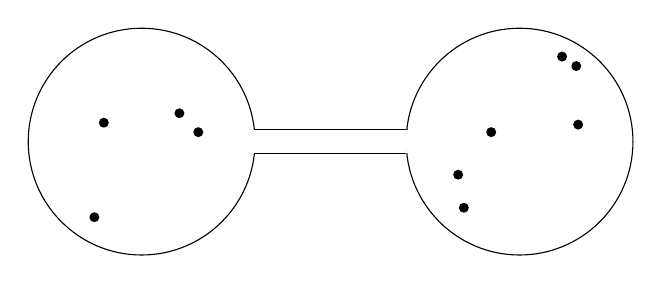
\begin{tikzpicture}[scale=1.2]
\draw (0,0) node {} circle[radius=1.2];
\draw[white,thick] (-6:1.2) arc(-6:6:1.2);
\draw (-6:1.2) -- +(1.63,0);
\draw (6:1.2) -- +(1.63,0);
\fill (-.4,.2) circle[radius=1.5pt];
\fill (.4,.3) circle[radius=1.5pt];
\fill (-.5,-.8) circle[radius=1.5pt];
\fill (.6,.1) circle[radius=1.5pt];
\begin{scope}[xshift=4cm]
\draw (0,0) node {} circle[radius=1.2];
\draw[white,thick] (174:1.2) arc(174:186:1.2);
\fill (-.3,.1) circle[radius=1.5pt];
\fill (.45,.9) circle[radius=1.5pt];
\fill (-.65,-.35) circle[radius=1.5pt];
\fill (.62,.18) circle[radius=1.5pt];
\fill (-.59,-.7) circle[radius=1.5pt];
\fill (.6,.8) circle[radius=1.5pt];
\end{scope}
\end{tikzpicture}
\end{center}
Repeated choose a particle at random with uniform distribution and move it to the other container. If there are $i$ particles in the left container then the probability of choosing a particle from the left container is $i/n$ and the probability of choosing a particle from the right container is $(n-i)/n$. If one container is empty the next particle must be chosen from the other container. 

The problem is similar to the gambler's ruin except that: (a) the process never ends and (b) the probability of a left or right step changes with each step:
\begin{center}
\begin{tikzpicture}[scale=1.2]
\draw (0,0) node[above left] {$A$} -- 
      (10,0) node[above right] {$B$};
\foreach \x in {0,1,2,3,4,5,6,7,8,9,10} {
  \draw (\x,0) -- +(0,4pt);
  \node at (\x,-10pt) { $\x$ };
}
\node at (4,-9mm) {$i$};
\node at (10,-9mm) {$n$};
\draw[fill] (4,7mm) circle[radius=1pt];
\draw[->] (4,7mm) -- node[above,xshift=-8pt] {$(n-i)/n$} +(-1,0);
\draw[->] (4,7mm) -- node[above,xshift=2pt] {$i/n$} +(1,0);
\draw[->] (0,7mm) -- node[above] {$1$} +(1,0);
\draw[<-] (9,7mm) -- node[above] {$1$} +(1,0);
\end{tikzpicture}
\end{center}

\subsection{Theoretical results}

The process is a Markov chain which eventually reaches a \emph{stationary distribution}:
\[
s_i=\dischoose{n}{i}\left(\frac{1}{n}\right)^n\,,
\]
where $s_i$ is the proportion of time that the particle is at the $i$'th position.

\subsection{Running the simulations}

The program asks the user how to run the simulation: with the saved value of $n$ or with a new value of $n$. Here is an output of the simulation:
\begin{verbatim}
Total particles in urns = 10
Theoretical stationary distribution
[0.001 0.01  0.044 0.117 0.205 0.246 0.205 0.117 0.044 0.01  0.001]
Simulation stationary distribution
[0.001 0.009 0.044 0.12  0.208 0.243 0.205 0.121 0.042 0.008 0.001]
\end{verbatim}
A graph of these distributions is shown in Figure~\ref{f.ehrenfest1}; the theoretical distribution and the result of simulation are so close together that the lines are slightly offset.

\begin{figure}
\begin{center}
\includegraphics[width=\textwidth]{ehrenfest-01}
\caption{Stationary distribution for the Ehrenfest model}\label{f.ehrenfest1}
\end{center}
\end{figure}

%%%%%%%%%%%%%%%%%%%%%%%%%%%%%%%%%%%%%%%%%%%%%%%%%%%%%%%%%%%%%%%%%%%%%

\section{The two-state process}\label{s.two-state}

The two-state process is similar to the Ehrenfest model in that the probabilities at each step are different and we are interested in the stationary probability distribution of the unbounded process. There are two states $A,B$. In state $A$ the process transitions to $B$  with probability $a$ and remains in $A$ with probability $1-a$. Similarly, the probability of a transition from $B$ to $A$ is $b$ and the probability of remaining in $B$ is $1-b$.
\begin{center}
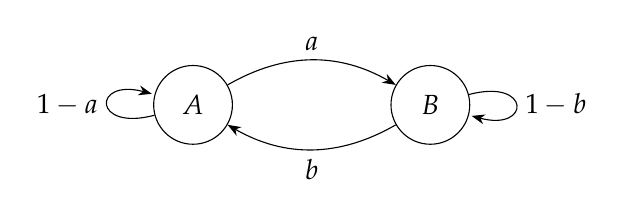
\begin{tikzpicture}[->,node distance = 6mm and 2cm]
\node[draw,circle,minimum size=10mm] (A) {$A$};
\node[draw,circle,minimum size=10mm] (B) [right=of A] {$B$};
\draw (A) edge[bend left] node[above] {$a$} (B);
\draw (B) edge[bend left] node[below] {$b$} (A);
\draw (A) edge [loop left] node {$1-a$} (A);
\draw (B) edge [loop right] node {$1-b$} (B);
\end{tikzpicture}
\end{center}
The stationary distribution, that is, the proportion of visits to $A$ and to $B$ is:
\[
\left[\frac{b}{a+b}, \frac{a}{a+b}\right]\,.
\]
Here is an output of a simulation:
\begin{verbatim}
Probabilities:  a = 0.500, b = 0.333
Theoretical stationary distribution: A = 0.400, B = 0.600
Simulation  stationary distribution: A = 0.402, B = 0.598
\end{verbatim}
When $a+b=1$ the probability of being at $A$ is $b$ and the probability of being at $B$ is $a$:
\begin{verbatim}
Probabilities:  a = 0.333, b = 0.667
Theoretical stationary distribution: A = 0.667, B = 0.333
Simulation  stationary distribution: A = 0.674, B = 0.326
\end{verbatim}
You can enter a required proportion $p$ of visits to $B$ and any probability $0<a<p$. The proportion will be achieved for:
\[
b = \frac{a(1-p)}{p}\,,
\]
as shown in the following simulation where we entered $p=0.8, a=0.6$:
\begin{verbatim}
Probabilities:  a = 0.600, b = 0.150, proportion = 0.800
Theoretical stationary distribution: A = 0.200, B = 0.800
Simulation  stationary distribution: A = 0.194, B = 0.806
\end{verbatim}


%%%%%%%%%%%%%%%%%%%%%%%%%%%%%%%%%%%%%%%%%%%%%%%%%%%%%%%%%%%%%%%%%%%%%

\section{The two-state process}\label{s.two-state}

The two-state process is similar to the Ehrenfest model in that the probabilities at each step are different and we are interested in the stationary probability distribution of the unbounded process. There are two states $A,B$. In state $A$ the process transitions to $B$  with probability $a$ and remains in $A$ with probability $1-a$. Similarly, the probability of a transition from $B$ to $A$ is $b$ and the probability of remaining in $B$ is $1-b$.
\begin{center}
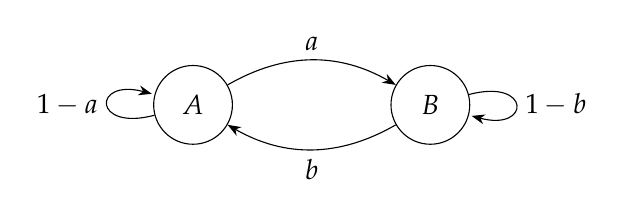
\begin{tikzpicture}[->,node distance = 6mm and 2cm]
\node[draw,circle,minimum size=10mm] (A) {$A$};
\node[draw,circle,minimum size=10mm] (B) [right=of A] {$B$};
\draw (A) edge[bend left] node[above] {$a$} (B);
\draw (B) edge[bend left] node[below] {$b$} (A);
\draw (A) edge [loop left] node {$1-a$} (A);
\draw (B) edge [loop right] node {$1-b$} (B);
\end{tikzpicture}
\end{center}
The stationary distribution, that is, the proportion of visits to $A$ and to $B$ is:
\[
\left[\frac{b}{a+b}, \frac{a}{a+b}\right]\,.
\]
Here is an output of a simulation:
\begin{verbatim}
Probabilities:  a = 0.500, b = 0.333
Theoretical stationary distribution: A = 0.400, B = 0.600
Simulation  stationary distribution: A = 0.402, B = 0.598
\end{verbatim}
When $a+b=1$ the probability of being at $A$ is $b$ and the probability of being at $B$ is $a$:
\begin{verbatim}
Probabilities:  a = 0.333, b = 0.667
Theoretical stationary distribution: A = 0.667, B = 0.333
Simulation  stationary distribution: A = 0.674, B = 0.326
\end{verbatim}
You can enter a required proportion $p$ of visits to $B$ and any probability $0<a<p$. The proportion will be achieved for:
\[
b = \frac{a(1-p)}{p}\,,
\]
as shown in the following simulation where we entered $p=0.8, a=0.6$:
\begin{verbatim}
Probabilities:  a = 0.600, b = 0.150, proportion = 0.800
Theoretical stationary distribution: A = 0.200, B = 0.800
Simulation  stationary distribution: A = 0.194, B = 0.806
\end{verbatim}

%%%%%%%%%%%%%%%%%%%%%%%%%%%%%%%%%%%%%%%%%%%%%%%%%%%%%%%%%%%%%%%%%%%%%

\newpage

\addcontentsline{toc}{section}{References}

\bibliographystyle{plain}
\bibliography{markov}

%%%%%%%%%%%%%%%%%%%%%%%%%%%%%%%%%%%%%%%%%%%%%%%%%%%%%%%%%%%%%%%%%%%%%

\end{document}
